\documentclass[a4paper]{elsarticle}

%% Language and font encodings
\usepackage[frenchb]{babel}
\usepackage[utf8x]{inputenc}
\usepackage[T1]{fontenc}
\usepackage{inconsolata}

\usepackage{xcolor}
\definecolor{pblue}{rgb}{0.13,0.13,1}
\definecolor{pgreen}{rgb}{0,0.5,0}
\definecolor{pred}{rgb}{0.9,0,0}
\definecolor{pgrey}{rgb}{0.46,0.45,0.48}

\usepackage{listings}
\lstdefinestyle{java}{language=Java,
  moredelim=[il][\textcolor{pgrey}]{$$},
  moredelim=[is][\textcolor{pgrey}]{\%\%}{\%\%}
}
\lstdefinestyle{sql}{language=SQL}

\lstdefinestyle{xml}{language=XML,
  morestring=[b]",
  morestring=[s]{>}{<},
  morecomment=[s]{<?}{?>},
  morekeywords={dependency,groupId,artifactId,version}
}
\lstset{style=java,
  literate={á}{{\'a}}1 {ã}{{\~a}}1 {é}{{\'e}}1,
  showspaces=false,
  showtabs=false,
  breaklines=true,
  showstringspaces=false,
  breakatwhitespace=true,
  commentstyle=\color{pgreen},
  keywordstyle=\color{pblue},
  stringstyle=\color{pred},
  aboveskip={1.3\baselineskip},
  basicstyle=\small\ttfamily\linespread{4},
  columns=flexible,
  extendedchars=true,
  frame=single,
  identifierstyle=\color{black},
  numbers=left,
  numberstyle=\scriptsize,
  prebreak = \raisebox{0ex}[0ex][0ex]{\ensuremath{\hookleftarrow}},
  showstringspaces=false,
  upquote=true
}

%% Sets page size and margins
\usepackage[a4paper,top=3cm,bottom=2cm,left=3cm,right=3cm,marginparwidth=1.75cm]{geometry}

%% Useful packages
\usepackage{amsmath}
\usepackage{amsfonts}
\usepackage{graphicx}
\usepackage[colorinlistoftodos]{todonotes}
\usepackage[colorlinks=true, allcolors=blue]{hyperref}

\newcommand{\norm}[1]{\left\lVert#1\right\rVert}

% https://tex.stackexchange.com/questions/312004/french-with-elsarticle-cls
\usepackage{regexpatch}
\makeatletter
\xpatchcmd{\abstract}{Abstract}{\abstractname}{}{}
\regexpatchcmd*{\@makecaption}{:}{\cA:}{}{}
\xpatchcmd*{\keyword}{Keywords}{Mots cl\'es}{}{}
\regexpatchcmd*{\keyword}{:}{\cA:}{}{}
\xpatchcmd{\printFirstPageNotes}
  {Email addresses}
  {Adresses email}
  {}{}
\xpatchcmd{\printFirstPageNotes}
  {Email address}
  {Adresse email}
  {}{}
\regexpatchcmd*{\printFirstPageNotes}{:}{\cA:}{}{}
\regexpatchcmd*{\ps@pprintTitle}% <cmd>
  {.*}% <search>
  {}% <replace>
  {}{}% <succes><failure>
\makeatother
\usepackage{silence}
\WarningFilter{frenchb.ldf}{Figure}

\usepackage{xspace}

% http://www.texample.net/tikz/examples/assignment-structure/
\usepackage{tikz}
\usetikzlibrary{calc,trees,positioning,arrows,chains,shapes.geometric,%
    decorations.pathreplacing,decorations.pathmorphing,shapes,%
    matrix,shapes.symbols}

\tikzset{
>=stealth',
  punktchain/.style={
    rectangle, 
    rounded corners, 
    % fill=black!10,
    draw=black, very thick,
    text width=20em, 
    minimum height=3em, 
    text centered, 
    on chain},
  line/.style={draw, thick, <-},
  element/.style={
    tape,
    top color=white,
    bottom color=blue!50!black!60!,
    minimum width=8em,
    draw=blue!40!black!90, very thick,
    text width=10em, 
    minimum height=3.5em, 
    text centered, 
    on chain},
  every join/.style={->, thick,shorten >=1pt},
  decoration={brace},
  tuborg/.style={decorate},
  tubnode/.style={midway, right=2pt},
}



\title{RV01 - Réalité virtuelle\\Projet VRXplore}
\author{Maurice QUACH -  Fabien BOUCAUD\\Automne 2017}

\begin{document}
\begin{frontmatter}
\address{Université de Technologie de Compiègne, France\vspace{1cm}
\begin{center}
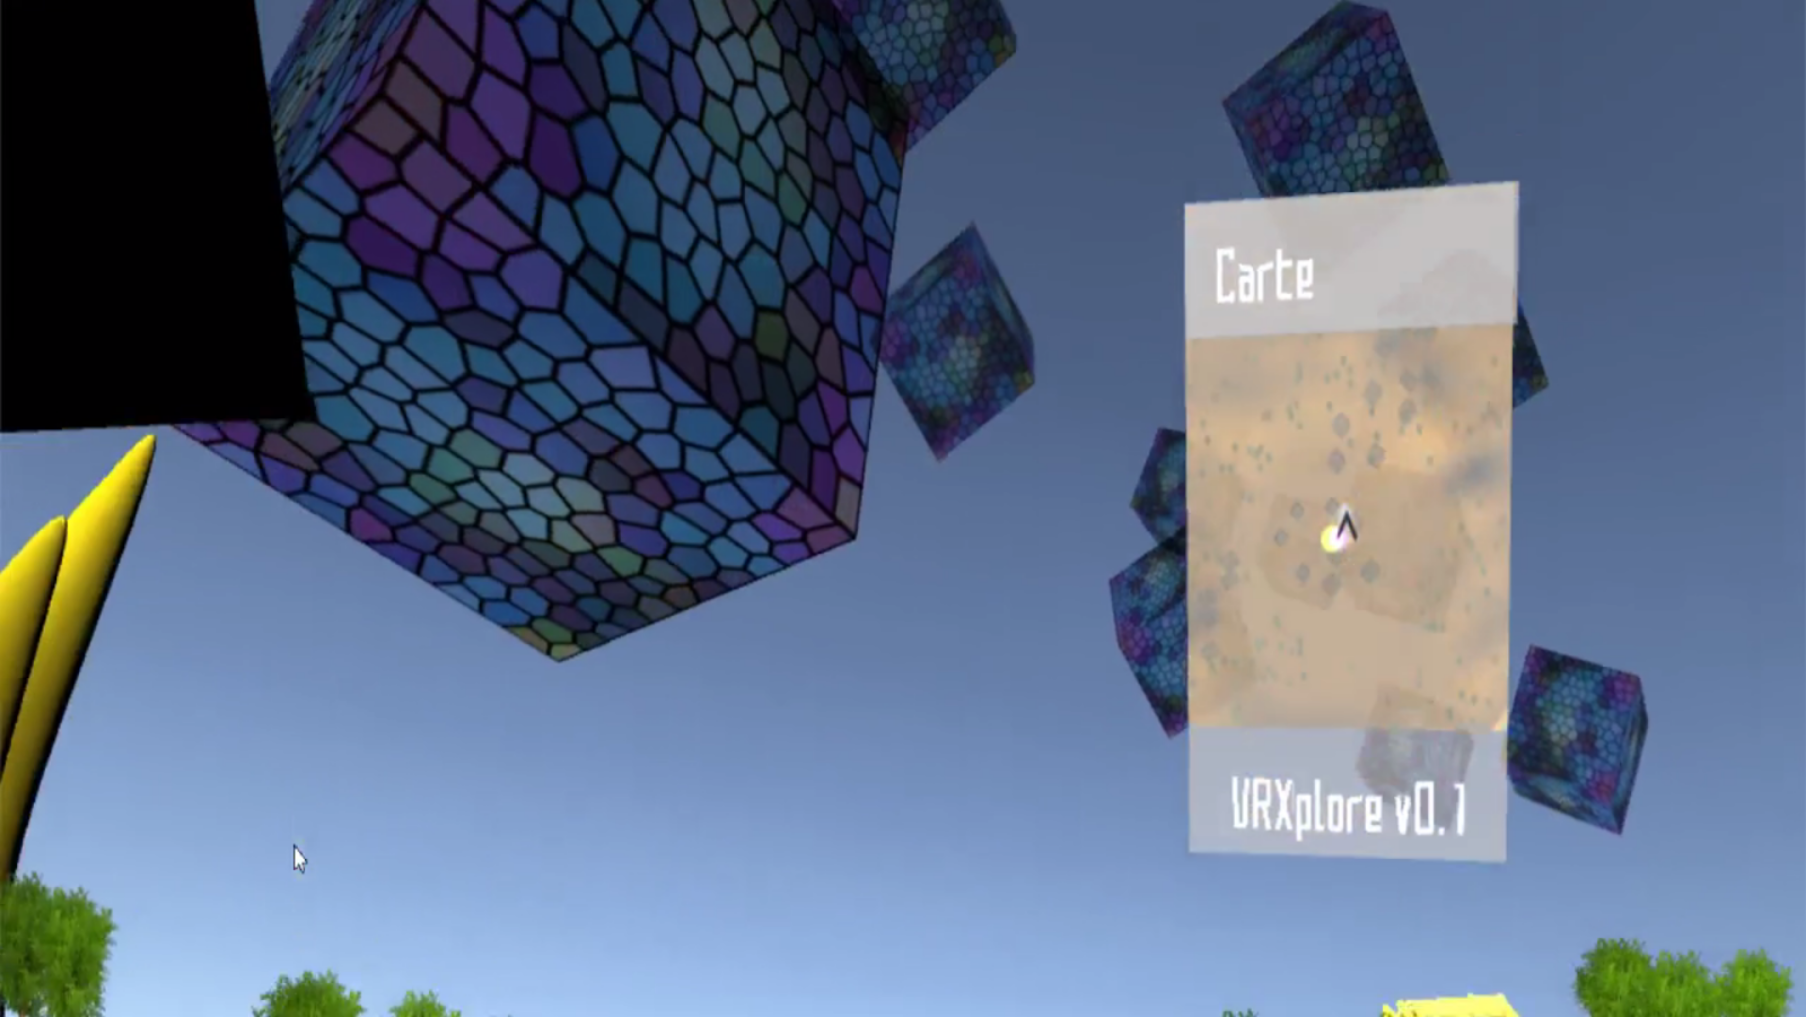
\includegraphics[width=\textwidth]{image_vrxplore.png}
\end{center}
\vspace{-1cm}}

\begin{abstract}

VRxplore est un projet réalisé dans le cadre de l’enseignement de réalité virtuelle RV01 proposé à l’UTC par Mme. Indira Thouvenin. Cet enseignement constitue une introduction aux principes et techniques de la réalité virtuelle. Cette introduction est mise en pratique par des travaux dirigés dédiés à Unity et surtout par la réalisation en petits groupes d’un projet de réalité virtuelle dont VRxplore est le fruit.

    VRxplore est une expérience d’exploration libre en réalité virtuelle d’un petit monde ouvert, au moyen d’une méthode de déplacement inhabituelle: le  \og grappin \fg{}.

\end{abstract}
\end{frontmatter}

\section{Contexte}

\subsection{Equipe et encadrants}

VRxplore fut réalisé par deux étudiants en fin de cursus à l’UTC (5ème semestre de Génie Informatique), Maurice Quach et Fabien Boucaud, et encadré par l’équipe enseignante de RV01 et en particulier Mme. Indira Thouvenin, M. Romain Guyard et M. Samba Drame.
    
Aucun des deux étudiants n’avaient d’expérience préalable ni avec Unity ni avec la réalisation d’applications en réalité virtuelle et tout fut donc appris et découvert au cours du semestre.

\subsection{Ressources}

Parmi les nombreuses ressources de réalité virtuelle et réalité augmentée mises à disposition des étudiants pour leurs projets RV01 par l’UTC (le Cave, les casques, la table de RA, etc.), nous avons choisi d’utiliser les casques HTC Vive et leurs dispositifs de pointage pour réaliser notre projet VRxplore. Il nous a en effet semblé qu’il s’agissait là du meilleur moyen de réaliser une expérience d’exploration et navigation totalement immersive avec possibilité de regarder et se déplacer tout autour de soi. Le projet fut développé sous Unity (version 5.6.3f) en utilisant à la fois nos ordinateurs personnels et ceux de l’UTC pour le développement.


\section{Objectif}

\subsection{Idée initiale}

Lors de la rédaction du cahier des charges pour le projet, nous avions l’ambition de réaliser une expérience immersive d’exploration d’un monde constitué de plateformes flottant dans le vide où l’utilisateur pourrait se déplacer de l’une à l’autre à l’aide d’un système de grappin. Il pourrait également pousser, prendre et tirer des objets et certaines plateformes proposeraient des énigmes basées sur ces interactions et parfois des altérations perceptives (modification des couleurs, plus de vision, etc.)
    
Nous avions beaucoup d’idées pour beaucoup d’éléments d’interaction, et nous nous sommes vite rendus compte lors du développement que ça en faisait en réalité trop pour un semestre et souvent pour des résultats peu intéressants.
    
\subsection{Resserrement du projet et résultat final}

A la suite de la première revue de développement du projet, nous avons donc choisi de resserrer le coeur du projet sur ce qui nous intéressait le plus de développer: le système de déplacement par grappin. En découle l’idée pour le résultat final du projet: une application d’exploration d’un petit monde ouvert en réalité virtuelle qui pousse au maximum l’utilisation d’un système de déplacement inhabituel, le grappin.
    
Ce resserrement nous a permis d’avoir un objectif de développement et de travail clair et de pouvoir aller le plus loin possible dans notre réflexion sur ce qui fait un moyen de déplacement réussi en réalité virtuel: ne pas rendre malade l’utilisateur, lui permettre de naviguer avec aisance, l’aider à ne pas se perdre par rapport à son environnement, l’aider à se localiser en permanence par rapport au monde, lui apporter des retours perceptifs liés à ses mouvements.


\section{Fonctionnalités}
\subsection{Le monde}

L’idée d’un monde uniquement constitué de plateformes flottant dans le vide fut abandonnée au profit d’un monde ouvert simple avec un peu de relief et des arbres, ainsi que quatre éléments particuliers: un gigantesque cube, un gigantesque cylindre, un labyrinthe flottant et une montagne. Enfin, pour offrir un terrain de jeu intéressant et propice à l’utilisation des grappins, une multitude d’\og îles \fg{}, des cubes colorés flottant, se trouvent un peu partout dans le monde, dans les airs.
    
Nous avons essayé de rendre une atmosphère visuelle à la fois un peu chaleureuse et un peu étrange, pas inquiétante mais hors du commun, de sorte à appuyer la distinction entre la réalité virtuelle et la  \og vraie \fg{}  réalité, et ainsi montrer que tout peut devenir possible dans cet autre univers. Même se déplacer en  \og grappin \fg{} .

\subsection{Le grappin}

A l’aide de chacun de ses dispositifs de pointage, l’utilisateur peut pointer n’importe quel élément du décor puis appuyer sur la gâchette du dispositif avec lequel il pointe pour placer son grappin. Pour confirmer perceptivement l’action, un effet sonore indique à l’utilisateur que son grappin a été lancé, et un effet de flash lumineux situé au point où le grappin est ancré permet de bien voir l’endroit où il se dirige. Suite à cela, il se retrouvera en effet attiré vers le point de l’espace où est accroché son grappin avec un léger effet de balancement et un gain de vitesse proportionnel à la distance à laquelle se trouve le grappin. On démarre lentement le déplacement et on gagne de la vitesse au fur et à mesure. En fonction de cette vitesse, on peut entendre un effet de vent plus ou moins fort (plus fort à mesure qu’on accélère), qui permet à l’utilisateur de se sentir d’autant mieux appartenir au monde.

Si l’utilisateur utilise à nouveau son même dispositif de pointage pour placer son grappin, l’ancre est dynamiquement déplacée au nouveau point choisi et l’utilisateur se retrouvera attiré vers ce nouveau point. Cela peut être réalisé à la volée même au milieu du déplacement pour ajuster sa trajectoire ou changer sa direction. En revanche, si on utilise le deuxième dispositif de pointage pour placer une ancre, nous serons également attiré vers ce deuxième point d’ancrage du grappin: les forces appliquées à l’avatar de l’utilisateur le feront donc osciller entre ces deux points de l’espace selon la distance entre eux. Utiliser les deux grappins à peu près au même endroit de l’espace peut permettre de démarrer et accélérer son déplacement plus rapidement.

Le déplacement est limité en terme de vitesse maximal à une valeur qui ne risque pas de rendre malade l’utilisateur, nos tests ayant montré qu’une très grande vitesse donnait facilement la nausée, en plus d’être difficilement manoeuvrable à la volée.

\subsection{Localisation et métaphore de navigation}

Avec le grappin en mode de déplacement, et compte tenu de l’effet de balancement, il peut arriver qu’on manque sa cible et qu’on se retrouve trop haut ou trop loin par rapport à ce qu’on visait, au moins pour un temps. Cela peut alors engendrer pour l’utilisateur une perte de repères spatiaux et le faire se sentir perdu par rapport à l’univers virtuel. Pour éviter ce problème qui peut être très désagréable et déboussolant pour l’utilisateur, voire favoriser la sensation de malaise/nausée, nous avons travaillé à fournir des moyens de se localiser en permanence à l’utilisateur.

La première chose mise en place fut les éléments du décor de grande échelle: le grand cube, le grand cylindre, la montagne et le labyrinthe, placé chacun à l’équivalent d’une position cardinale dans le monde virtuel. Ces repères visuels sont suffisamment imposants pour rester facilement visible à l’utilisateur aussi loin ou aussi haut qu’il se retrouve entraîné, et ainsi lui éviter une perte de repère. Ce n’est toutefois pas un système infaillible, et nous avons donc choisi de rajouter une métaphore de localisation/navigation sous la forme d’une mini-carte que l’utilisateur peut choisir d’afficher ou non sur une partie de son champ de vision en appuyant sur le trackpad de son dispositif de pointage gauche.

L’idée initiale de la mini-carte nous est venue en partant de l’élément qui nous semblait le plus signifiant en termes de déplacement dans notre application: l’ancre du grappin. Nous avons donc dans un premier temps fait une sorte de radar qui indiquait notre position au centre et deux indicateurs colorés qui indiquaient la position relative des deux ancres de nos grappins (si elles sont ancrées dans le monde). Cela permet de toujours garder à l’esprit notre position relative à l’endroit vers lequel on voulait initialement se diriger et avoir une idée de notre distance par rapport à ce point et de la direction vers laquelle se tourner pour pouvoir de nouveau le voir. A cela s’est rajoutée l’idée de mettre une représentation du monde miniature sous forme de carte pour avoir en plus une idée générale de notre position et de celle de nos ancres dans le monde. Toutefois, la carte était dans un premier temps fixe et seul notre position était mise à jour lors de nos déplacements, ce qui n’est pas forcément évident pour se repérer, d’autant moins en VR, puisqu’il faut faire l’effort de se replacer mentalement par rapport à l’orientation de la carte. Nous avons donc eu l’idée de modifier l’orientation de la carte et avec elle la position des ancres dynamiquement en fonction du regard de l’utilisateur, de sorte que la carte soit toujours orientée avec les choses qu’on a devant nous vers le haut, et derrière nous vers le bas. Cela rend beaucoup plus aisée et instinctive l’utilisation et la compréhension de la carte.

\subsection{Autres}

Quelques autres éléments d’interactions qui avaient été commencés pendant le développement restent utilisables mais sans grand intérêt. On peut pousser les quelques cubes qui se trouvent là où l’utilisateur apparaît en utilisant le trackpad du dispositif de pointage droit en visant le cube et en étant assez proche. Cela a aussi pour effet de pousser l’utilisateur en arrière, qui est un effet de contrecoup sur lequel on avait commencé à réfléchir avant de resserrer le projet sur le déplacement.

Il est également possible, une fois dans le labyrinthe flottant, de viser les murs avec les dispositifs de pointage et d’utiliser les grips en les serrant dans nos mains pour sentir les murs via un retour vibratoir si on en est assez proche. Nous voulions en effet proposer d’explorer un labyrinthe plongé dans le noir en ne pouvant se repérer qu’au  \og toucher \fg{}  des murs via les vibrations. La fonctionnalité ne marche pas très bien et a également été abandonnée lors du resserrement du projet sur le déplacement par grappin.

\section{Développement}

\subsection{Difficultés rencontrées}

Si VRxplore peut, à la lecture de ce rapport, sembler simple dans ses objectifs et son fonctionnement, il n’en fut pas moins difficile à réaliser et il nous fallut surmonter de nombreux problèmes.

D’abord, comme mentionné précédemment, ni l’un ni l’autre des membres de l’équipe n’avait jamais travaillé ni avec Unity ni avec la réalité virtuelle, et il fallut donc beaucoup nous renseigner et demander de l’aide au cours du développement, ce qui nous a assurément ralenti.

Plus important, notre idée originale pour le projet comportait beaucoup d’éléments différents, et nous avons eu du mal pendant longtemps à déterminer la priorité à donner aux fonctionnalités et savoir vers quoi avancer et travailler. C’est d’autant plus vrai qu’il ne s’agit pas ici d’un jeu où il est facile de voir quel est l’objectif (qu’il soit narratif ou lié aux règles du gameplay et son implémentation). Ce n’est qu’au moment de la revue de projet de mi-développement et suite aux remarques de l’équipe encadrantes qu’il a été choisi de se re-concentrer sur le déplacement par grappin et que nous avons alors pu beaucoup plus facilement savoir sur quoi avancer.

Nous avons dû passer beaucoup de temps sur la calibration des formules de force à ajouter à l’avatar lors du placement du grappin, car le déplacement rendait très rapidement malade. Garder le casque même vingt ou trente secondes donnait la nausée à cause de trop forts balancements, d’une trop grande vitesse de déplacement, etc. Une grande partie du travail fut donc de calibrer les formules de calcul des forces pour rendre l’expérience agréable.

La mini-carte fut également  longue à élaborer et bien implémenter, puisqu’il a fallu travailler sur les matrices de rotation pour avoir une carte dynamique dans son orientation en fonction du regard de l’utilisateur. La gestion de la caméra aérienne à partir de laquelle nous générons la carte demanda également un peu de temps de prise en main et de travail.

Enfin, nous avons également essayé de travailler le rendu graphique, puisque dans un premier temps nous avions trop de ressources et d’éléments, ce qui rendait la compilation extrêmement longue voire impossible, et l’application connaissait parfois des ralentissements. En essayant de jouer sur les shaders et les effets visuels pour réduire le nombre et la qualité des éléments tout en offrant un rendu visuel agréable à l’oeil et une ambiance intéressante, nous nous sommes heurtés à beaucoup de problèmes liés à la réalité virtuelle et l’utilisation du casque.

Ces difficultés furent néanmoins très enrichissantes car elles nous ont permis de vraiment prendre en conscience de ce que cela implique que de travailler en réalité virtuelle et d’offrir une expérience de qualité dans cet environnement, ce que nous pensons avoir relativement réussi, malgré la présence d’encore quelques bugs.

\subsection{Développement de la physique du grappin}

La chaîne du grappin attire le joueur vers la destination en utilisant le moteur physique d'Unity. Nous décrivons ici les itérations principales qui nous ont amenées à la version finale.

Soit $d$ la destination du joueur, $p$ position initiale du joueur à un instant $t$ et $a$ une constante correspondant à la force d'attraction (définie à 1000 dans le projet).
On adopte la notation suivante pour la normalisation d’un vecteur :

\begin{equation}
\hat{u} = \frac{u}{|u|}
\end{equation}

On définit les vecteur $w$ et $k$ à un instant $t$ :

\begin{equation}
w = d - p
\end{equation}
\begin{equation}
k = \hat{w}
\end{equation}

On note $v$ la vitesse du joueur à un instant $t$.

On note $F$ la force appliquée au joueur à intervalle régulier (FixedUpdate).

\subsubsection{Version initiale}

Notre version initiale est très simple. Elle est fonctionnelle mais présente le problème d'être extrêmement difficile à contrôler.

La prise de vitesse est longue dans un premier temps puis la vitesse augmente de façon très importante. Le joueur dépasse très souvent la destination pour ensuite y être ramené d'une manière similaire. Cela résulte en un \og effet pendule \fg{} très important.

Un mécanisme d'arrêt a été mis en place pour arrêter le joueur lorsqu'il arrive à la destination. Ce mécanisme était peu efficace car il nécessite d'être proche de la destination ce qui est difficile.

La conséquence est que le contrôle est difficile et que le joueur a rapidement la nausée. Lors de nos tests, il était difficile de tenir plus de 5 secondes avec le casque.

\begin{equation}
    F = 
\begin{cases}
    k * a,& \text{si } |w| \geq 1\\
    0,              & \text{sinon}
\end{cases}
\end{equation}

\subsubsection{Prise en compte de la distance}

Dans cette seconde version, l'idée est de prendre en compte la distance de manière plus importante. La force est importante lorsque la distance est grande et se réduit lorsque l'on se rapproche de la destination.

L'amélioration est importante par rapport à la version initiale. Le contrôle est beaucoup plus aisé. Cependant, \og l'effet pendule \fg{} reste non négligeable et il est difficile de tenir plus de 30 secondes avec le casque lorsque l'on réalise des déplacements complexes.

\begin{equation}
    F = 
\begin{cases}
    k * (1 - e^{-|w|}) * a,& \text{si } |w| \geq 1\\
    0,              & \text{sinon}
\end{cases}
\end{equation}

\subsubsection{Force multi-composantes}

Dans cette troisième version, nous avons adopté une approche un peu différente. Nous avons tenté de créer une force à plusieurs composantes afin d'arriver au résultat désiré.

Cette version est bien plus aisée à contrôlée et le confort utilisateur est amélioré. Il est possible de l'utiliser pendant 5 minutes sans problème. \og L'effet pendule \fg{} est cependant toujours présent dans un nombre non négligeable de situations.

Nous définissons alors trois forces :
\begin{itemize}
\item Force d'attraction : attire l'utilisateur vers la destination
\item Force anti-gravité : rend le \og démarrage/décollage \fg{} plus aisé et atténue \og l'effet pendule \fg{} dû à la gravité
\item Force de stabilisation : atténue \og l'effet pendule \fg{} dû à l'accumulation de vitesse
\end{itemize}

La force d'attraction reste la même que précédemment.

\begin{equation}
    F_{attraction} = k * (1 - e^{-|w|}) * a
\end{equation}

La force d'anti-gravité est forte lorsque la distance est grande afin de \og démarrer/décoller \fg{} plus rapidement. Elle se réduit lorsque l'on se rapproche afin de ne pas amplifier \og l'effet pendule \fg{}.

\begin{equation}
    F_{antigrav} = (0, 1, 0) * 10 * (1 - e^{-|w|})
\end{equation}

Soit $x$ la direction de stabilisation définie par :
\begin{equation}
    x = (d - (p + v))
\end{equation}

La direction de stabilisation atténue \og l'effet pendule \fg{} en utilisant la vitesse de l'utilisateur pour compenser de manière préemptive. On supprime la force de stabilisation sur l'axe vertical car cela amplifie \og l'effet pendule \fg{}.

\begin{equation}
    F_{stab} = \left( {\begin{array}{ccc}
   1 & 0 & 0\\
   0 & 0.5 & 0\\
   0 & 0 & 1\\
  \end{array} } \right) * e^{-|w|} * \hat{x} * (a / 2)
\end{equation}

\begin{equation}
    F = 
\begin{cases}
    F_{attraction} + F_{antigrav} + F_{stab},& \text{si } |w| \geq 1\\
    0,              & \text{sinon}
\end{cases}
\end{equation}

\subsubsection{Correction de l'effet pendule}

Après analyses et tests, nous avons réussi à atténuer grandement \og l'effet pendule \fg{} sans le supprimer. En effet, c'est une partie intégrante du mécanisme de déplacement mais il est important qu'il ne dégrade pas l'expérience utilisateur en étant trop important, causant alors un inconfort.

Afin d'arriver au résultat voulu, nous avons \og adouci \fg{} l'exponentielle en utilisant la fonction racine carrée. En rouge, $1-e^{-x}$ et en bleu $1-e^{-\sqrt{x}}$.

\begin{center}
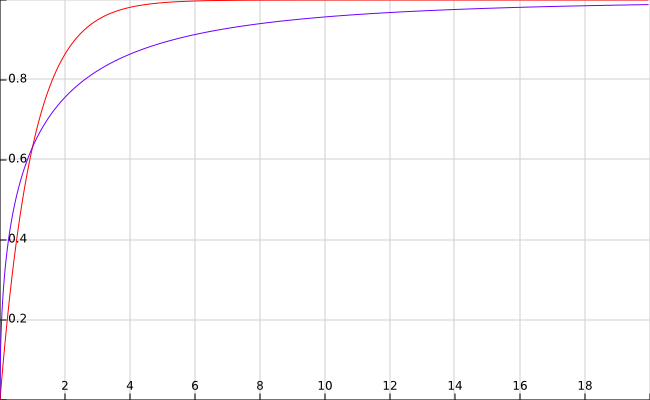
\includegraphics[width=0.8\textwidth]{exp_sqrt.png}
\end{center}

Le système de force est identique à celui défini précédemment. Par contre, les formules pour la force d'attraction et la force de stabilisation sont modifiées de la manière suivante.

\begin{equation}
    F_{attraction} = k * (1 - e^{-\sqrt{|w|}}) * a
\end{equation}

Pour la force de stabilisation, nous ajoutons la racine carrée et nous divisons la distance par 3 afin de diminuer l'impact de la distance sur la stabilisation. En bleu, $1-e^{-\sqrt{x / 3}}$ et en rouge $1-e^{-x}$.

\begin{center}
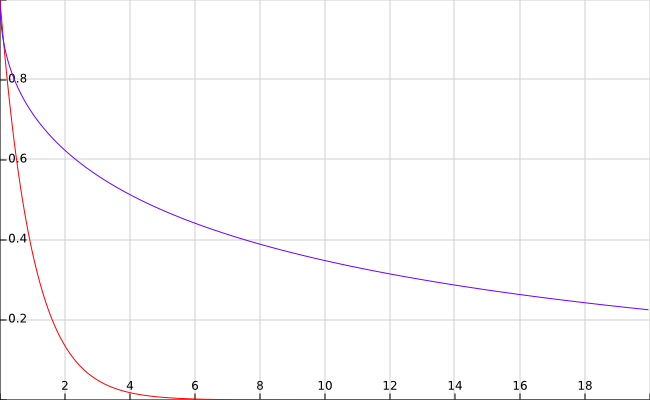
\includegraphics[width=0.8\textwidth]{exp_sqrt_3_non_3.png}
\end{center}

On multiplie aussi la force de stabilisation par la vitesse à la puissance 1.5 divisée par 5. Après tests, nous avons observé que la puissance 1 était insuffisante et que la puissance 2 était trop importante. La valeur 5 a été obtenue après des tests pour déterminer la valeur fournissant le meilleur confort.

\begin{equation}
    F_{stab} = \left( {\begin{array}{ccc}
   1 & 0 & 0\\
   0 & 0.5 & 0\\
   0 & 0 & 1\\
  \end{array} } \right) * e^{-\sqrt{|w| / 3}} * \hat{x} * a * (|v|^{1.5} / 5)
\end{equation}

\subsection{Volume du vent en fonction de la vitesse}

Pour le volume du vent, nous avons utilisé la formule suivante afin d'avoir une indication sonore de la vitesse utilisateur. Cela participe à l'immersion et le réalisme.

Pour un volume entre 0 et 1, nous avons utilisé la formule suivante.

\begin{equation}
volume = max\left(0.05, \frac{min(1, max(0, |v| - 10) / 40)^{2}}{2}\right)
\end{equation}

\subsection{Niveau de réalisation}

Etant donné la grande évolution du projet en terme d’objectif, les niveaux de réalisation proposés au moment du cahier des charges ne sont plus vraiment totalement applicables à notre projet. Toutefois, nous estimons avoir réussi à fournir un travail d’une bonne qualité en termes de gestion du déplacement, de sa physique et de ses retours perceptifs, de sorte que l’on peut naviguer aisément, sans se perdre ni être trop inquiété par le fait d’être malade. Nous estimons que nous nous trouvons donc plutôt entre le niveau intermédiaire et le niveau maximal de réalisation, quelques manques existant encore pour avoir une expérience vraiment très agréable et réaliste, mais le niveau actuel nous semblant déjà très satisfaisant.

\subsection{Possibilités d’améliorations}

En termes d’amélioration, nous aurions souhaité avoir un peu plus de temps pour peaufiner les retours sonores, ajouter des bruits de collision de l’avatar avec l’environnement, notamment avec les objets qu’il risque de heurter en utilisant le grappin, et en affinant encore un peu le son du vent en fonction de la vitesse de déplacement (jouer sur l’altitude par exemple).

Il reste également quelques bugs à régler et éléments à ajuster dont le plus important: la carte disparaît (c’est-à-dire devient noire) parfois selon la direction dans laquelle l’utilisateur regarde et sa position, probablement à cause de notre implémentation de la caméra qui gère la mini-carte.
Dans l’ensemble, notre travail nous apparaît comme un bon point de départ pour ensuite aller plus loin et intégrer ce moyen de déplacement dans un monde et un ensemble d’interactions plus poussées.

\section{Conclusion}

En conclusion, ce projet RV01 fut une très bonne expérience d’apprentissage des principes et techniques de la réalité virtuelle. Nous avons notamment pu monter en compétence sur Unity et nous rendre compte de ce qui est possible et moins possible avec la réalité virtuelle, des éléments auxquels il faut faire attention pour rendre l’expérience agréable et réaliste pour l’utilisateur, et de ce que la réalité virtuelle peut apporter.

Ce fut un travail passionnant pour lequel nous aurions aimé avoir plus de temps, étant donné que nous sommes plutôt contents de ce que nous avons déjà réalisé et que nous aurions aimé pouvoir encore peaufiner et améliorer cette expérience.


%%\section*{Bibliographie}

%%\bibliographystyle{elsarticle-num}
%%\bibliography{sample}

\end{document}